\section{Movimiento uniforme}

\subsection{Definición}
El movimiento uniforme es aquel en el cual la velocidad es constante en el tiempo.
\vspace{-20pt}

\begin{align*}
\vec{v}_x = \text{cte} \quad \Rightarrow \quad \vec{a} = 0
\end{align*}

\vspace{-20pt}

\subsection{Velocidad}
\vspace{-20pt}

\begin{align*}
\vec{v}_x &= \frac{\Delta \vec{x}}{\Delta t} \\
\Delta \vec{x} &= \vec{v}\,\Delta t
\end{align*}

Si $\Delta t$ es constante, entonces también $\Delta x$ es constante.

\vspace{-10pt}

\subsection{Ecuación de movimiento}
\vspace{-30pt}

\begin{align*}
\vec{x}_f - \vec{x}_0 &= \vec{v}_x (t_f - \cancel{t_0}) \\
\text{Tomando } t_f = t: \\
\Aboxed{\vec{x}_f &= \vec{x}_0 + \vec{v}_x t} \quad \text{(ecuación vectorial)} \\
\Aboxed{x &= x_0 + v_x t} \quad \text{(ecuación escalar)}
\end{align*}

\subsection{Interpretación gráfica}

\begin{figure}[H]
    \centering
    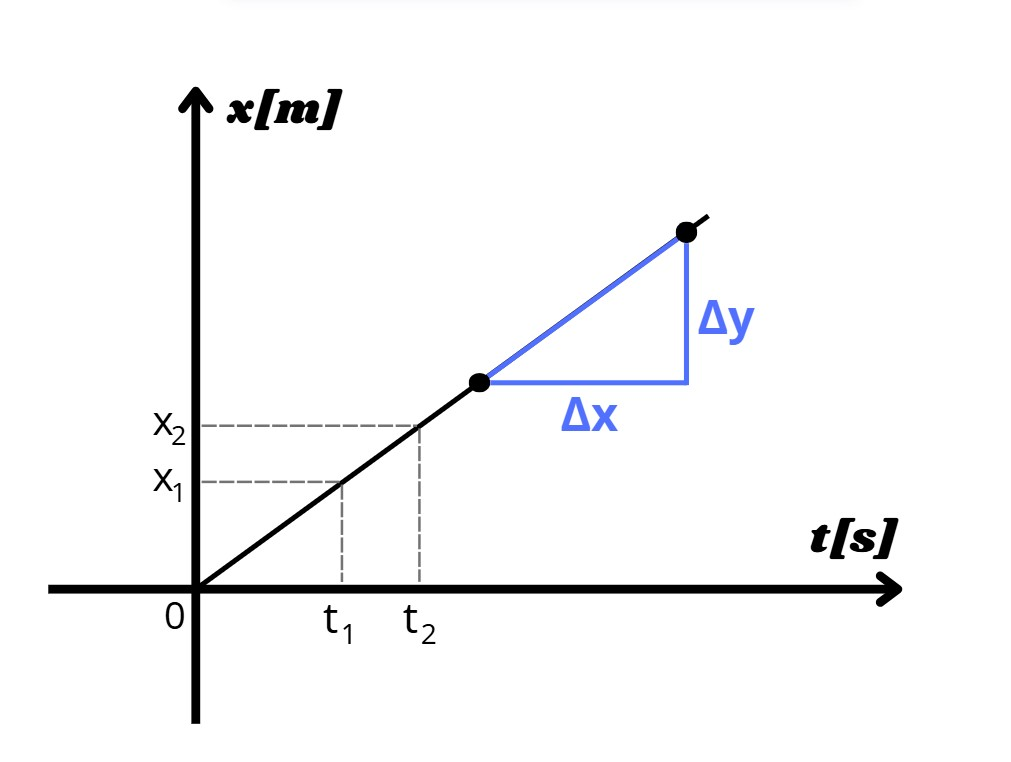
\includegraphics[width=0.6\textwidth]{images/demonstrations/uniformMovement.jpg}
    \caption{Representación gráfica del movimiento uniforme}
\end{figure}

La ecuación es de la forma:
\vspace{-20pt}

\begin{align*}
\vec{r} &= \vec{r_0} + \vec{v}t\\
y &= A + Bx
\end{align*}

Donde:
\begin{itemize}
\item $A$ es la ordenada en el origen ($x_0$)
\item $B$ es la pendiente ($v = \frac{\Delta x}{\Delta t}$)
\end{itemize}